\documentclass[a4paper, 12pt]{article}
\usepackage[utf8x]{inputenc}
\usepackage[english, russian]{babel}
\usepackage[left=25mm, top=25mm, right=25mm, bottom=25mm]{geometry}
\usepackage{cmap}
\usepackage{indentfirst}
\usepackage{tikz}
\usepackage{float}
\usepackage{amsmath, amsfonts, amssymb}
\usepackage{graphicx}
\usepackage{hyperref}
\usepackage{listings}
\usepackage{caption}
\usepackage{subcaption}
\usepackage{xcolor}
\usepackage{etoolbox}
\usepackage{titlesec}
\pagestyle{plain}
\patchcmd{\tableofcontents}{\contentsname}{\centering\contentsname}{}{}
\titleformat{\section}[block]{\normalfont\large\bfseries\centering}{}{0pt}{}
\titleformat{\subsection}[block]{\normalfont\normalsize\bfseries\centering}{}{0pt}{}
\allowdisplaybreaks
\graphicspath{{src/images/}}
\usetikzlibrary{patterns}
\definecolor{LightGray}{gray}{0.95}
\definecolor{LightGray2}{gray}{0.7}
\lstdefinestyle{code}{
    language=MATLAB, % replace language here
    basicstyle=\footnotesize\ttfamily,
    % numbers=left,
    % numberstyle=\scriptsize\color{gray},
    % stepnumber=1,
    % numbersep=5pt,
    backgroundcolor=\color{LightGray},
    showspaces=false,
    showstringspaces=false,
    showtabs=false,
    tabsize=4,
    captionpos=b,
    breaklines=true,
    breakatwhitespace=false,
    frame=single,
    rulecolor=\color{LightGray2},
    linewidth=\linewidth,
    keywordstyle=\color{blue}\bfseries,
    commentstyle=\color{green!40!black},
    stringstyle=\color{purple},
    escapeinside={\%*}{*)},
    inputencoding=utf8x,
    xleftmargin=0pt,
    framexleftmargin=0pt,
    framexrightmargin=0pt
}
\lstset{style=code}
\hypersetup{
    colorlinks=true,
    linkcolor=blue,
    filecolor=magenta,
    urlcolor=cyan,
    pdftitle={contents setup},
    pdfpagemode=FullScreen,
}


\begin{document}
    \begin{titlepage}

        \begin{center}
        Федеральное государственное автономное образовательное учреждение высшего образования
        «Национальный Исследовательский Университет ИТМО»
        \vfill
        
        
\includegraphics[width=0.3\textwidth]{itmo.png} % requires /src/images/itmo.png

        {\large\bf ЛАБОРАТОРНАЯ РАБОТА №4}\\
        {\large\bf ПРЕДМЕТ «ТЕОРИЯ АВТОМАТИЧЕСКОГО УПРАВЛЕНИЯ»}\\
        {\large\bf ТЕМА «СЛЕЖЕНИЕ И КОМПЕНСАЦИЯ: ВИРТУАЛЬНЫЙ ВЫХОД»}\\
        Вариант №2
        \vfill

        \begin{flushright}
            \begin{minipage}{.45\textwidth}
            {
                \hbox{Преподаватель:}
                \hbox{Пашенко А. В.}
                \hbox{}
                \hbox{Выполнил:}
                \hbox{Румянцев А. А.}
                \hbox{}
                \hbox{Факультет: СУиР}
                \hbox{Группа: R3341}
                \hbox{Поток: ТАУ R22 бак 1.1.1}
            }
            \end{minipage}
        \end{flushright}
        \vfill
  
        Санкт-Петербург\\
        2025
        \end{center}
    \end{titlepage}
    
    \tableofcontents

    \newpage
    \section{Задание 1. Компенсирующий регулятор по состоянию}
    Рассмотрим систему
    $$
    \dot{x}=Ax+Bu+B_f w_f,
    $$
    $$
    A=\begin{bmatrix}
        5 &2 &7\\
        2 &1 &2\\
        -2 &-3 &-4
    \end{bmatrix},\ B=\begin{bmatrix}
        3\\1\\-1
    \end{bmatrix},\ B_f=\begin{bmatrix}
        -4 &0 &0 &-1\\
        0 &0 &0 &0\\
        4 &0 &0 &0
    \end{bmatrix},\ x(0)=\begin{bmatrix}
        0\\0\\0
    \end{bmatrix},
    $$
    генератор внешнего возмущения
    $$
    \dot{ w}_f=\Gamma w_f,\ \Gamma=\begin{bmatrix}
        25 &6 &-20 &11\\
        14 &3 &-10 &4\\
        40 &11 &-31 &17\\
        6 &4 &-4 &3
    \end{bmatrix},\  w_f(0)=\begin{bmatrix}
        1\\1\\1\\1
    \end{bmatrix}
    $$
    и виртуальный выход вида
    $$
    z=C_Zx,\ C_Z=\begin{bmatrix}
        -2 &1 &-1
    \end{bmatrix};
    $$

    
    \subsection{Характер внешнего возмущения}
    Для определения характера внешнего возмущения найдем собственные числа матрицы $\Gamma$.
    Программа в \texttt{MATLAB} находится на листинге \ref{task1} в приложении 1
    $$
    \sigma\left( \Gamma \right)=\left\{ \pm i, \pm 3i \right\}
    $$
    Так как спектр состоит только из мнимых собственных чисел, то характер возмущения -- гармоники
    без затухания и роста амплитуды с течением времени.


    \subsection{Схема моделирования системы, замкнутой компенсирующим регулятором}
    Построим схему моделирования системы, замкнутой компенсирующим регулятором
    $$u=K_1x+K_2 w_f,$$ обеспечивающим выполнение целевого условия $$\lim\limits_{t\to\infty}z(t)=0$$
    при внешнем воздействии, задаваемом генератором. Снимаем осциллограммы $u(t)$, $w_f(t)$, $x(t)$, $z(t)$
    \begin{figure}[H]
        \centering
        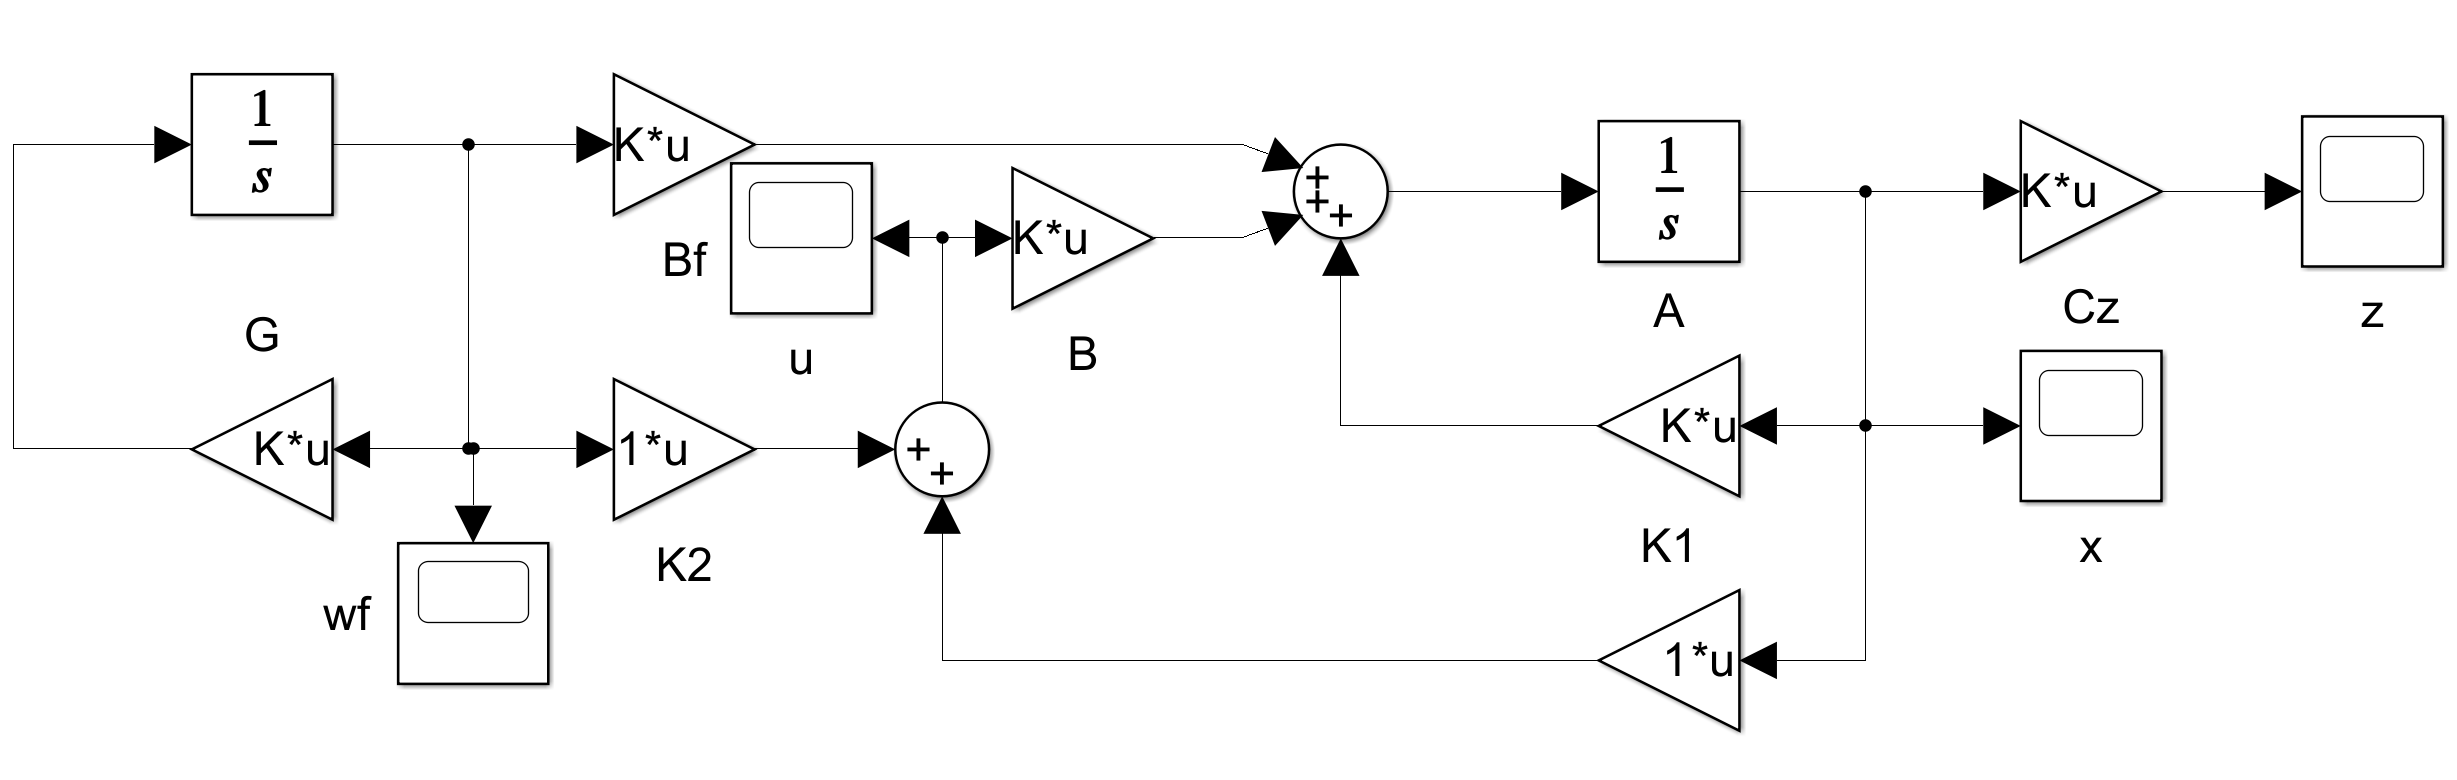
\includegraphics[scale=0.225]{1task_scheme.png}
        \captionsetup{skip=0pt}
        \caption{Схема моделирования системы, замкнутой компенсирующим регулятором}
        \label{fig:1task_scheme}
    \end{figure}


    \subsection{Исследование системы перед синтезом регулятора}
    Определим управляемость и стабилизируемость системы.
    Найдем собственные числа матрицы $A$
    $$
    \sigma\left( A \right)=\left\{ -2,2\pm i \right\}
    $$
    Собственное число $\lambda_1=-2$ асимптотически устойчивое, остальные неустойчивые.
    Выполним жорданово разложение матрицы $A$ в вещественной форме. Найдем вектор
    $B$ в базисе собственных векторов матрицы $A$. Получаем
    $$
    A_{J_{re}}=\begin{bmatrix}
    -2     &0     &0\\
    0     &2     &1\\
    0    &-1     &2
    \end{bmatrix},\ B_{J_{re}}=\begin{bmatrix}
    0\\
     3\\
    -1
    \end{bmatrix};
    $$
    Собственное число $\lambda_1=-2$ неуправляемое, остальные управляемые. Система не полностью управляема,
    стабилизируема. Максимальная степень устойчивости
    $\alpha=|\min{\left(\text{Re}\left( \tilde{\sigma}\left( A \right):\lambda_i\in\mathbb{C}_{-} \right)\right)}|=2$.


    \subsection{Синтез компоненты обратной связи компенсирующего регулятора}
    Синтезируем $K_1$ с помощью матричного уравнения типа Риккати
    $$
    A^TP+PA+Q-\nu PBR^{-1}B^TP+2\alpha P=0,\,K=-R^{-1}B^TP;
    $$
    Зададим
    $Q=0,\ \nu=2,\ R=1$. Решаем при $\alpha=2$. Получаем матрицу регулятора
    $$
    K_1=\begin{bmatrix}
    1.6000  &-11.2000    &1.6000
    \end{bmatrix}
    $$
    Проверим собственные числа замкнутой системы $A+BK_1$
    $$
    \sigma\left( A+BK_1 \right)=\left\{ -2,-2.0000 \pm 4.1231i \right\}
    $$
    Желаемая степень устойчивости достигнута, регулятор синтезирован корректно.


    \subsection{Синтез компоненты прямой связи компенсирующего регулятора}
    Чтобы синтезировать $K_2$, нужно найти $K_1$, найти $P,Y$
    как решение системы уравнений, после чего вычислить $K_2$ по формуле
    $$
    \begin{cases}
        P\Gamma-AP=BY+B_f,\\
        C_ZP+D_Z=0,
    \end{cases}\ K_2=Y-K_1P;
    $$
    Предоставим вычисления пакету \texttt{cvx} в \texttt{MATLAB}. Получаем
    $$
    K_2=\begin{bmatrix}
        -48.3631  &-13.0092   &35.7538  &-23.4769
    \end{bmatrix}
    $$


    % pos 885,224,768,358
    \subsection{Компьютерное моделирование}
    Выполним компьютерное моделирование разомкнутой системы $\left( u=0 \right)$;
    замкнутой регулятором только с $K_1$ компонентой; замкнутой компенсирующим регулятором.
    Построим графики вектора состояния генератора внешнего возмущения
    $ w_f(t)$, формируемого регулятором управления $u(t)$, вектора состояния объекта управления
    $x(t)$ и виртуального выхода $z(t)$.
    Результаты представлены на рис. \ref{fig:1task_wf}--\ref{fig:1task_zz}
    \begin{figure}[H]
        \centering
        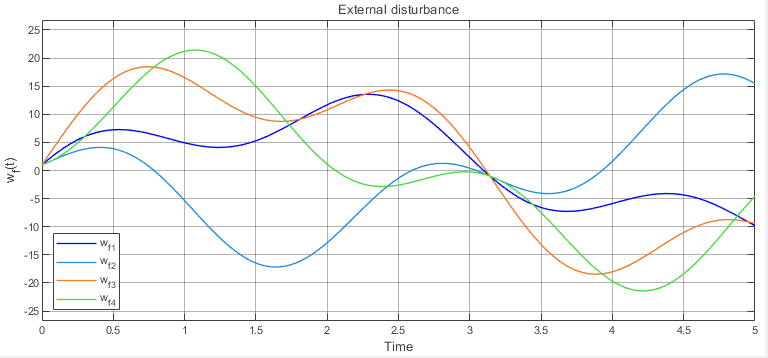
\includegraphics[scale=0.75]{1task_wf.png}
        \captionsetup{skip=0pt}
        \caption{График возмущений $ w_f(t)$}
        \label{fig:1task_wf}
    \end{figure}
    \begin{figure}[H]
        \centering
        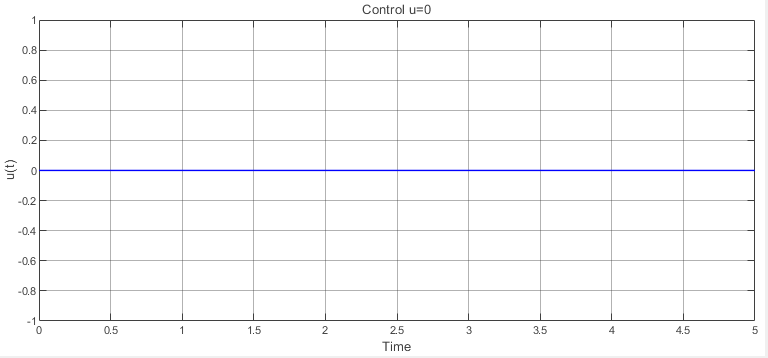
\includegraphics[scale=0.75]{1task_unull_u.png}
        \captionsetup{skip=0pt}
        \caption{График управления $u(t)=0$}
        \label{fig:1task_unull_u}
    \end{figure}
    \begin{figure}[H]
        \centering
        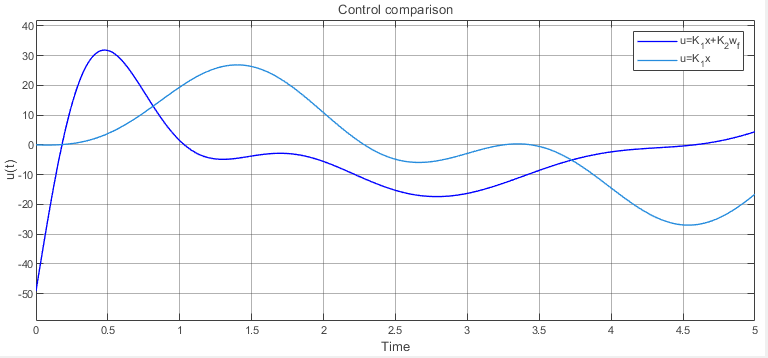
\includegraphics[scale=0.75]{1task_uu.png}
        \captionsetup{skip=0pt}
        \caption{График сравнения управлений $u(t)=K_1x$ и $u(t)=K_1x+K_2 w_f$}
        \label{fig:1task_uu}
    \end{figure}
    \begin{figure}[H]
        \centering
        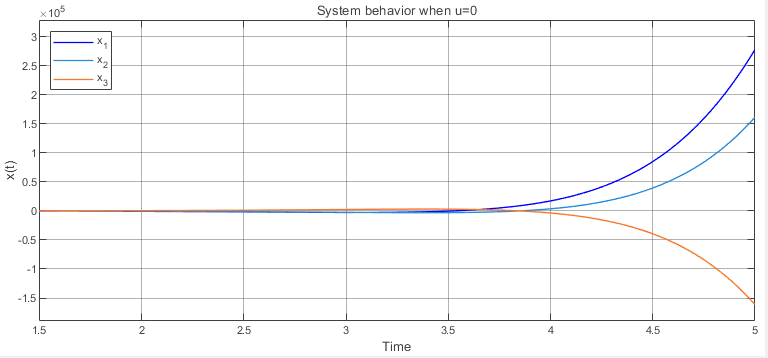
\includegraphics[scale=0.75]{1task_unull_x.png}
        \captionsetup{skip=0pt}
        \caption{График поведения системы $x(t)$ при $u(t)=0$}
        \label{fig:1task_unull_x}
    \end{figure}
    \begin{figure}[H]
        \centering
        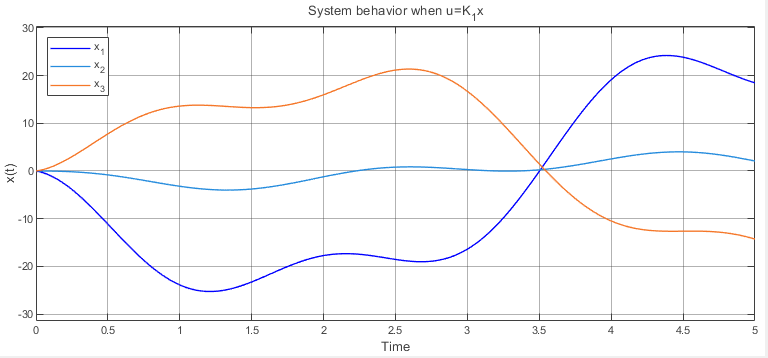
\includegraphics[scale=0.75]{1task_uk_x.png}
        \captionsetup{skip=0pt}
        \caption{График поведения системы $x(t)$ при $u(t)=K_1x$}
        \label{fig:1task_uk_x}
    \end{figure}
    \begin{figure}[H]
        \centering
        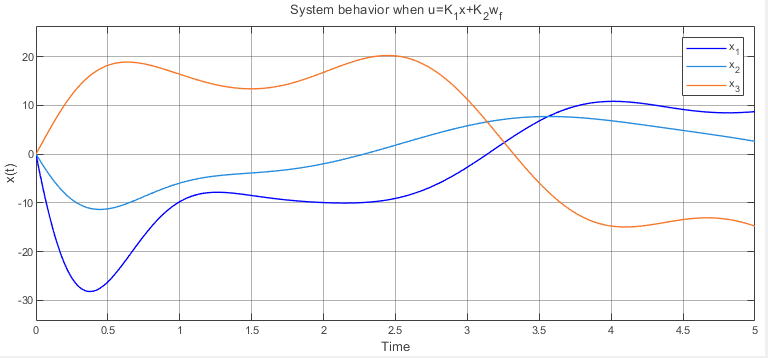
\includegraphics[scale=0.75]{1task_ukk_x.png}
        \captionsetup{skip=0pt}
        \caption{График поведения системы $x(t)$ при $u(t)=K_1x+K_2 w_f$}
        \label{fig:1task_ukk_x}
    \end{figure}
    \begin{figure}[H]
        \centering
        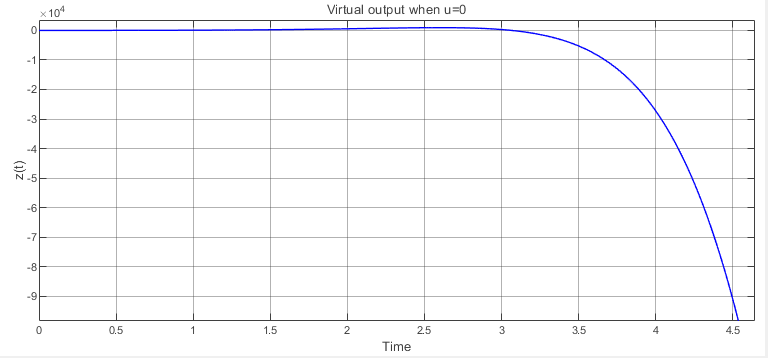
\includegraphics[scale=0.75]{1task_unull_z.png}
        \captionsetup{skip=0pt}
        \caption{График виртуального выхода $z(t)$ при $u(t)=0$}
        \label{fig:1task_unull_z}
    \end{figure}
    \begin{figure}[H]
        \centering
        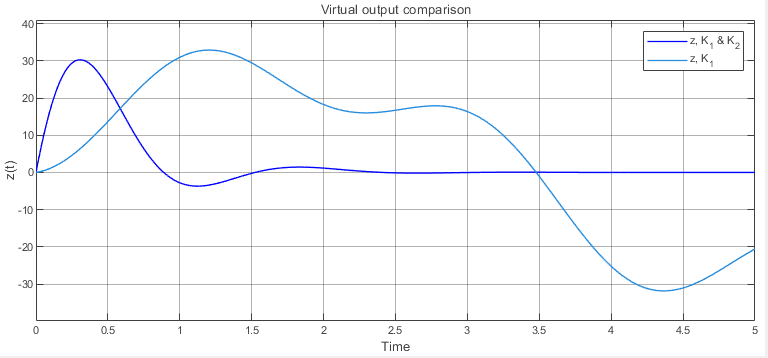
\includegraphics[scale=0.75]{1task_zz.png}
        \captionsetup{skip=0pt}
        \caption{График сравн. виртуальных выходов $z(t)$ при $u(t)=K_1x$ и $u(t)=K_1x+K_2 w_f$}
        \label{fig:1task_zz}
    \end{figure}
    \noindent Траектория $z(t)$ при компенсирующем регуляторе стремится к нулю -- регулятор выполнил свою задачу.
    При отсутствии $K_2$ компоненты $z(t)$ не стабилизируется, но и не расходится (см. рис. \ref{fig:1task_zz}). При разомкнутой системе
    виртуальный выход расходится (см. рис. \ref{fig:1task_unull_z}). При отсутствии управления вектор
    состояния объекта управления расходится, при наличии -- нет, но и не стабилизируется (см. рис. \ref{fig:1task_unull_x}, \ref{fig:1task_uk_x}, \ref{fig:1task_ukk_x}).
    При наличии $K_2$ компоненты регулятор сразу начинает действовать на объект управления, при наличии только $K_1$ компоненты
    регулятор постепенно управляет системой (см. рис. \ref{fig:1task_uu}).


    \subsection{Вывод}
    В данном задании был исследован компенсирующий регулятор по состоянию.
    Был синтезирован компенсирующий регулятор. Было проведено компьютерное
    моделирование при различных конфигурациях регулятора.
    Результаты были сравнены. Компенсирующий регулятор был синтезирован корректно.


    \section{Задание 2. Следящий регулятор по состоянию}
    Рассмотрим систему (матрицы $A,B,C_Z,\Gamma$ такие же, как в задании 1)
    $$
    \dot{x}=Ax+Bu,\ x(0)=\begin{bmatrix}
        1 &1 &1
    \end{bmatrix}^T,
    $$
    генератор задающего сигнала
    $$
    \dot{ w}_g=\Gamma w_g,\  w_g(0)=\begin{bmatrix}
        1 &1 &1 &1
    \end{bmatrix}^T
    $$
    и виртуальный выход вида
    $$
    z=C_Zx+D_Z w_g,\ D_Z=\begin{bmatrix}
        -20 &-6 &16 &-9
    \end{bmatrix};
    $$


    \subsection{Характер внешнего возмущения}
    Матрица $\Gamma$ такая же, как в первом задании. Ее спектр имеет вид
    $$
    \sigma\left( \Gamma \right)=\left\{ \pm i, \pm 3i \right\}
    $$
    Характер возмущений -- гармоники без затухания и роста амплитуды с течением времени.


    \subsection{Схема моделирования системы, замкнутой следящим регулятором}
    Построим схему моделирования системы, замкнутой следящим регулятором
    $$
    u=K_1x+K_2 w_g,
    $$
    обеспечивающим выполнение целевого условия
    $$\lim\limits_{t\to\infty}z(t)=0$$
    при внешнем воздействии, задаваемом генератором. Снимаем осциллограммы $u(t)$, $w_g(t)$, $x(t)$, $z(t)$
    \begin{figure}[H]
        \centering
        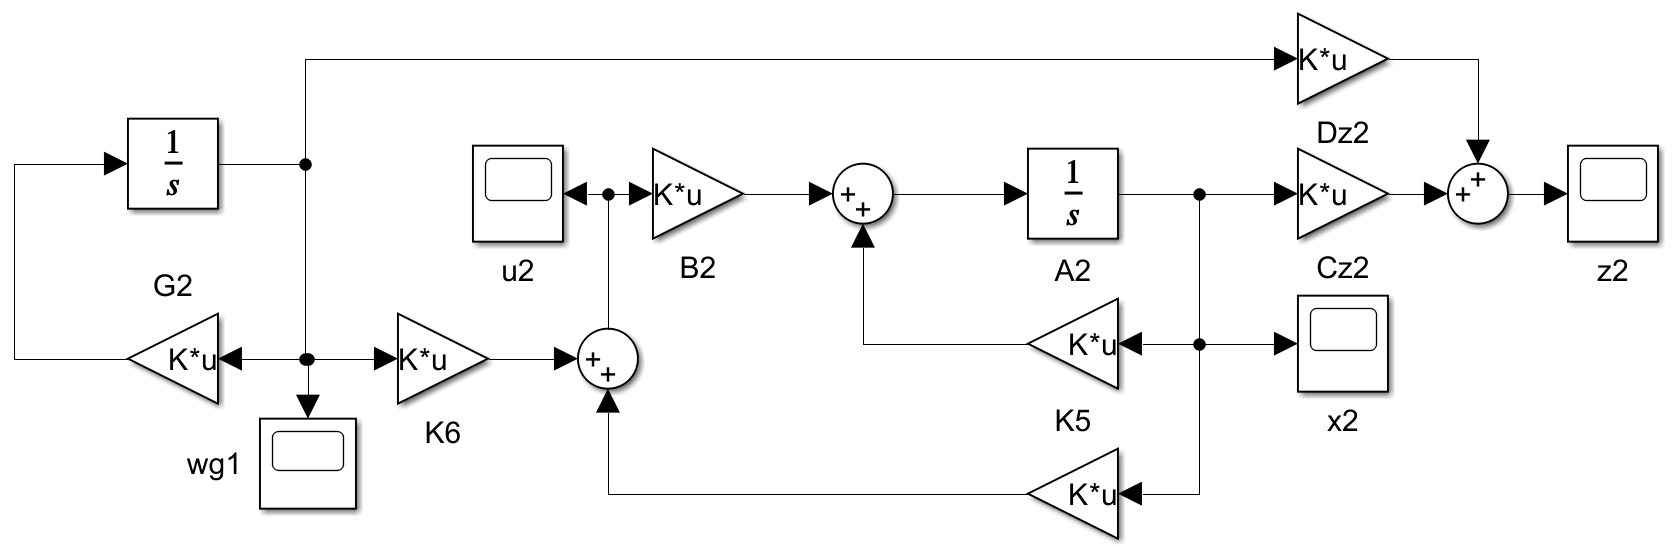
\includegraphics[scale=0.325]{2task_scheme.png}
        \captionsetup{skip=0pt}
        \caption{Схема моделирования системы, замкнутой следящим регулятором}
        \label{fig:2task_scheme}
    \end{figure}


    \subsection{Исследование системы перед синтезом регулятора}
    Матрицы $A,B$ такие же, как в первом задании. Имеем
    $$
    \sigma\left( A \right)=\left\{ -2,2\pm i \right\},\ A_{J_{re}}=\begin{bmatrix}
        -2     &0     &0\\
        0     &2     &1\\
        0    &-1     &2
        \end{bmatrix},\ B_{J_{re}}=\begin{bmatrix}
        0\\
         3\\
        -1
        \end{bmatrix};
    $$
    Система не полностью управляема, стабилизируема. Максимальная степень устойчивости $\alpha=2$.


    \subsection{Синтез компоненты обратной связи следящего регулятора}
    Синтезируем $K_1$ так же, как в задании 1 -- с помощью матричного уравнения Риккати.
    Матрицы, участвующие в расчетах, не изменились. Таким образом, имеем
    $$
    K_1=\begin{bmatrix}
    1.6000  &-11.2000    &1.6000
    \end{bmatrix},\
    \sigma\left( A+BK_1 \right)=\left\{ -2,-2.0000 \pm 4.1231i \right\};
    $$
    В первом задании уже выяснили, что регулятор синтезирован корректно.


    \subsection{Синтез компоненты прямой связи следящего регулятора}
    Синтезируем $K_2$ аналогично заданию 1. Из системы уравнений пропадет $B_f$, взамен появится $D_Z$.
    Программа представлена на листинге \ref{task2} в приложении 2. Получаем
    $$
    K_2=\begin{bmatrix}
        7.2    &3.2  &-8.0  &4.0
    \end{bmatrix}
    $$


    \subsection{Компьютерное моделирование}
    Выполним компьютерное моделирование систем аналогично заданию 1
    \begin{figure}[H]
        \centering
        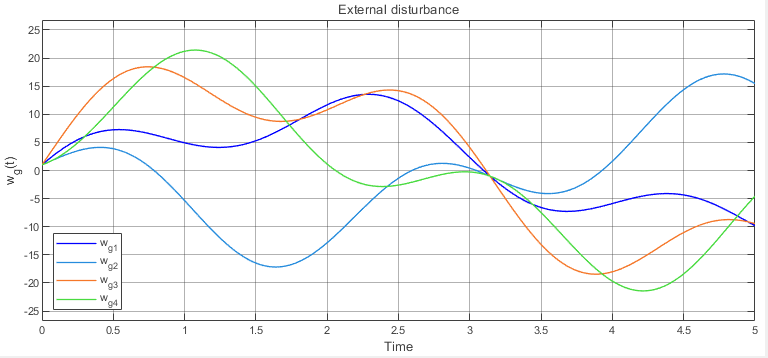
\includegraphics[scale=0.75]{2task_wg.png}
        \captionsetup{skip=0pt}
        \caption{График возмущений $ w_g(t)$}
        \label{fig:2task_wg}
    \end{figure}
    \begin{figure}[H]
        \centering
        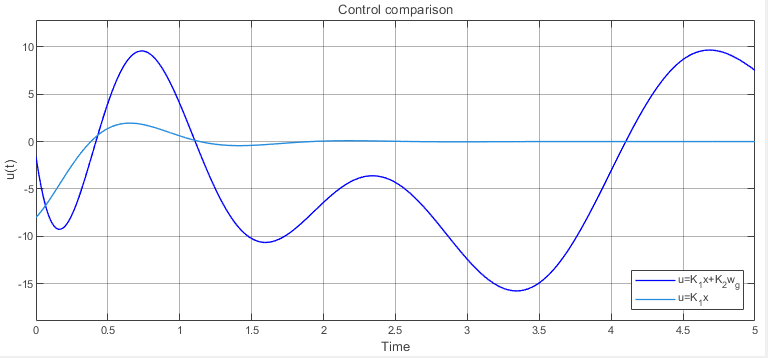
\includegraphics[scale=0.75]{2task_uu.png}
        \captionsetup{skip=0pt}
        \caption{График сравнения управлений $u(t)=K_1x$ и $u(t)=K_1x+K_2 w_g$}
        \label{fig:2task_uu}
    \end{figure}
    \begin{figure}[H]
        \centering
        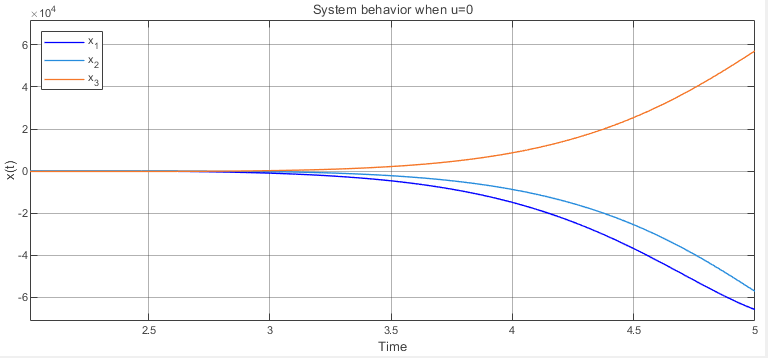
\includegraphics[scale=0.75]{2task_unull_x.png}
        \captionsetup{skip=0pt}
        \caption{График поведения системы $x(t)$ при $u(t)=0$}
        \label{fig:2task_unull_x}
    \end{figure}
    \begin{figure}[H]
        \centering
        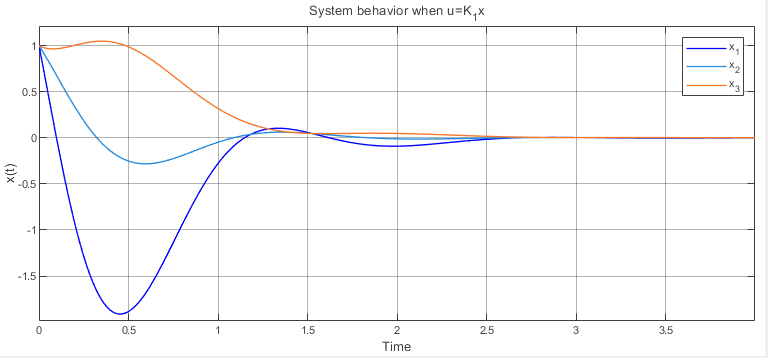
\includegraphics[scale=0.75]{2task_uk_x.png}
        \captionsetup{skip=0pt}
        \caption{График поведения системы $x(t)$ при $u(t)=K_1x$}
        \label{fig:2task_uk_x}
    \end{figure}
    \begin{figure}[H]
        \centering
        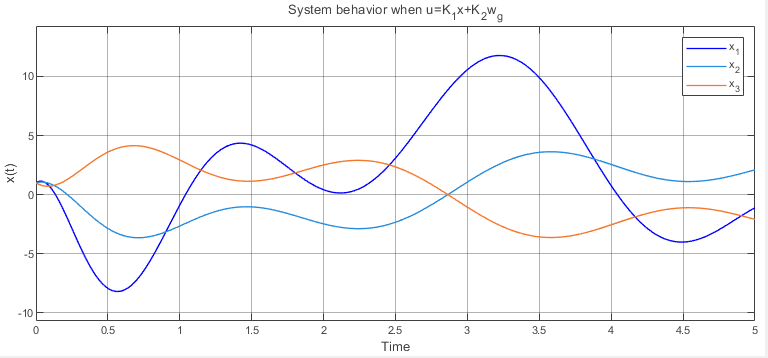
\includegraphics[scale=0.75]{2task_ukk_x.png}
        \captionsetup{skip=0pt}
        \caption{График поведения системы $x(t)$ при $u(t)=K_1x+K_2 w_g$}
        \label{fig:2task_ukk_x}
    \end{figure}
    \begin{figure}[H]
        \centering
        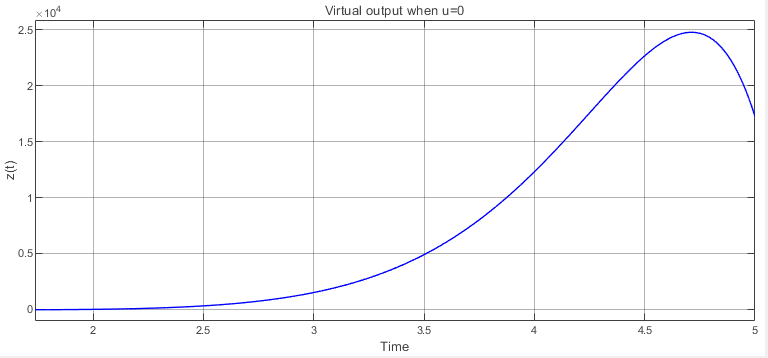
\includegraphics[scale=0.75]{2task_unull_z.png}
        \captionsetup{skip=0pt}
        \caption{График виртуального выхода $z(t)$ при $u(t)=0$}
        \label{fig:2task_unull_z}
    \end{figure}
    \begin{figure}[H]
        \centering
        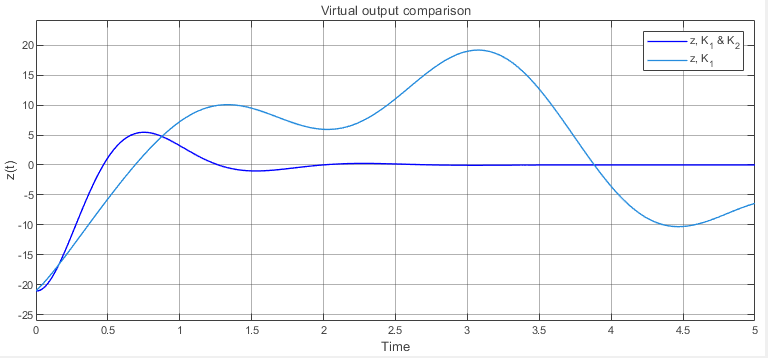
\includegraphics[scale=0.75]{2task_zz.png}
        \captionsetup{skip=0pt}
        \caption{График сравн. виртуальных выходов $z(t)$ при $u(t)=K_1x$ и $u(t)=K_1x+K_2 w_g$}
        \label{fig:2task_zz}
    \end{figure}
    \noindent Следящий регулятор выполнил свою задачу -- на рис. \ref{fig:2task_zz}
    $z(t)$ стремится к нулю с увеличением времени. Виртуальный выход для регулятора только
    с компонентой $K_1$ не расходится, но и не стабилизируется. При отсутствии управления $z(t)$
    расходится (см. рис. \ref{fig:2task_unull_z}). Вектор состояния объекта управления под действием
    регулятора только с $K_1$ компонентой стабилизируется к нулю, но виртуальный выход продолжает
    движение под действием внешних возмущений ($C_Zx\rightarrow0,D_Z w_g\nrightarrow0$).
    При наличии компонент $K_1,K_2$ график $x(t)$ не стабилизируется к нулю, но и не расходится (см. рис. \ref{fig:2task_ukk_x}),
    при этом $z(t)$ достигает целевого состояния. Без управления $x(t)$ расходится (см. рис. \ref{fig:2task_unull_x}).
    При наличии только компоненты $K_1$ управление со временем стабилизируется к нулю, при наличии обеих компонент -- нет (см. рис. \ref{fig:2task_uu}).


    \subsection{Вывод}
    В данном задании был исследован следящий регулятор по состоянию.
    Его синтез был проведен аналогично синтезу компенсирующего регулятора в задании 1.
    Было выполнено компьютерное моделирование систем со сравнением результатов.


    \section{Задание 3. Слежение и компенсация по выходу}
    Рассмотрим систему (матрицы $A,B,B_f,C_Z,D_Z$ такие же, как в предыдущих заданиях)
    $$
    \begin{cases}
        \dot{x}=Ax+Bu+B_f w,\\
        y=Cx+D w,
    \end{cases}\ x(0)=\begin{bmatrix}
        0 &0 &0
    \end{bmatrix}^T
    $$
    и генератор внешнего воздействия
    $$
    \dot{ w}=\Gamma w,\  w(0)=\begin{bmatrix}
        1 &1 &1 &1
    \end{bmatrix}^T
    $$
    при
    $$
    C=\begin{bmatrix}
        2 &0 &3
    \end{bmatrix},\ D=\begin{bmatrix}
        8 &2 &-6 &4
    \end{bmatrix};
    $$


    \subsection{Характер внешнего возмущения}
    Матрица $\Gamma$ такая же, как в предыдущих заданиях. Ее спектр
    содержит только мнимые числа.
    Характер возмущений -- гармоники
    без затухания и роста амплитуды с течением времени.


    \subsection{Возможность осуществления слежения и компенсации по выходу}
    Проверим пару $$\left(\begin{bmatrix}
        C &D
    \end{bmatrix},\begin{bmatrix}
        A &B_f\\
        0 &\Gamma
    \end{bmatrix}\right)$$ на обнаруживаемость. Обозначим
    $$
    \mathcal{C}=\begin{bmatrix}
        C &D
    \end{bmatrix},\ \mathcal{A}=\begin{bmatrix}
        A &B_f\\
        \mathbf{0_{4\times3}} &\Gamma
    \end{bmatrix};
    $$
    Найдем собственные числа матрицы $\mathcal{A}$. Программа в \texttt{MATLAB} представлена на листинге \ref{task3} в приложении 3
    $$
    \sigma\left( \mathcal{A} \right)=\left\{ -2,2\pm i,\pm i, \pm3i \right\}
    $$
    Собственное число $\lambda_1=-2$ асимптотически устойчивое, может быть ненаблюдаемым.
    Комплексные пары $\lambda_{4,5}=\pm i,\lambda_{6,7}=\pm3i$ устойчивые, но не асимптотически.
    Комплексная пара $\lambda_{2,3}=2\pm i$ неустойчивая, нужна наблюдаемость.
    Найдем вещественное жорданово разложение матрицы $\mathcal{A}$,
    а матрицу $\mathcal{C}$ переведем в базис собственных
    векторов матрицы $\mathcal{A}$. Получаем
    $$
    \mathcal{A}_{J_{re}}=\begin{bmatrix}
        -2         &0         &0    &0    &0   &0   &0\\
         0    &2    &1    &0    &0   &0   &0\\
         0   &-1    &2    &0    &0   &0   &0\\
         0         &0         &0         &0    &1         &0         &0\\
         0         &0         &0   &-1         &0         &0         &0\\
         0         &0         &0         &0         &0         &0    &3\\
         0         &0         &0         &0         &0   &-3         &0
    \end{bmatrix},\ \mathcal{C}_{J_{re}}=\begin{bmatrix}
        1.0000\\    1.0000\\         0.0000\\    0.9500\\    2.1500\\   -1.2192\\    0.5038
    \end{bmatrix}^T;
    $$
    Все жордановы клетки относятся к различным собственным числам.
    Для комплексной пары $\lambda_{2,3}=2\pm i$ в $\mathcal{C}_{J_{re}}$ один из двух
    соответствующих ей столбцов ненулевой, следовательно $\lambda_{2,3}$ наблюдаемы.
    Остальные собственные числа наблюдаемы.
    Таким образом, система полностью наблюдаема и обнаруживаема.
    Слежение и компенсация по выходу осуществимы.


    \subsection{Уравнение регулятора в форме Вход-Состояние-Выход}
    Найдем матрицу $\bar{A}$, которая будет нужна в дальнейшем для построения схемы
    и проведения вычислений, через запись уравнения регулятора в форме В-С-В, где
    вход это $y(t)$, а выход $u(t)$.
    Расширенный объект имеет вид
    \begin{align}
        \begin{cases}
            \dot{x}=Ax+Bu+B_f w,\\
            \dot{ w}=\Gamma w,\\
            y=Cx+D w,\\
            z=C_Zx+D_Z w;
        \end{cases} \label{eq:ext_obj}
    \end{align}
    Для него можно записать следящий регулятор по выходу
    \begin{align}
        \begin{cases}
            \dot{\hat{x}}=A\hat{x}+Bu+B_f\hat{w}+L_1\left( \hat{y}-y \right),\\
            \dot{\hat{w}}=\Gamma \hat{w}+L_2\left( \hat{y}-y \right),\\
            \hat{y}=C\hat{x}+D\hat{w},\\
            u=K_1\hat{x}+K_2\hat{w};
        \end{cases}\label{eq:uout}
    \end{align}
    Выполним подстановку $\hat{y},u$ в $\dot{\hat{x}}$ и выразим $\hat{x},\hat{w}$, чтобы позже
    вынести эти компоненты как вектор, на который умножается матрица $\bar{A}$. Аналогично с $y$. Имеем
    \begin{align}
        &\dot{\hat{x}}=A\hat{x}+Bu+B_f\hat{w}+L_1\left( \hat{y}-y \right), \notag\\
        &\dot{\hat{x}}=A\hat{x}+B\left( K_1\hat{x}+K_2\hat{w} \right)+B_f\hat{w}+L_1\left( C\hat{x}+D\hat{w}-y \right), \notag\\
        &\dot{\hat{x}}=A\hat{x}+BK_1\hat{x}+BK_2\hat{w}+B_f\hat{w}+L_1C\hat{x}+L_1D\hat{w}-L_1y, \notag\\
        &\dot{\hat{x}}=\left( A+BK_1+L_1C \right)\hat{x}+\left( BK_2+B_f+L_1D \right)\hat{w}-L_1y \label{eq:dot_x_est};
    \end{align}
    Проведем аналогичные действия для $\dot{\hat{w}}$
    \begin{align}
        &\dot{\hat{w}}=\Gamma \hat{w}+L_2\left( \hat{y}-y \right), \notag\\
        &\dot{\hat{w}}=\Gamma \hat{w}+L_2\left( C\hat{x}+D\hat{w}-y \right), \notag\\
        &\dot{\hat{w}}=\Gamma \hat{w}+L_2C\hat{x}+L_2D\hat{w}-L_2y, \notag\\
        &\dot{\hat{w}}=\left( L_2C \right)\hat{x}+\left( \Gamma+L_2D \right)\hat{w}-L_2y \label{eq:dot_w_est};
    \end{align}
    Запишем регулятор по выходу (\ref{eq:uout}) с учетом подстановок (\ref{eq:dot_x_est}), (\ref{eq:dot_w_est})
    \begin{align}
        \begin{cases}
            \dot{\hat{x}}=\left( A+BK_1+L_1C \right)\hat{x}+\left( BK_2+B_f+L_1D \right)\hat{w}-\left(L_1\right)y,\\
            \dot{\hat{w}}=\left( L_2C \right)\hat{x}+\left( \Gamma+L_2D \right)\hat{w}-\left(L_2\right)y,\\
            u=\left(K_1\right)\hat{x}+\left(K_2\right)\hat{w};
        \end{cases}\label{eq:temp_in_state_out}
    \end{align}
    Вынесем компоненты за скобками в соответствующие векторы
    \begin{align}
        \begin{cases}
            &\begin{bmatrix}
                \dot{\hat{x}}\\
                \dot{\hat{w}}
            \end{bmatrix}=\begin{bmatrix}
                A+BK_1+L_1C &BK_2+B_f+L_1D\\
                L_2C &\Gamma+L_2D
            \end{bmatrix}\begin{bmatrix}
                \hat{x}\\
                \hat{w}
            \end{bmatrix}-\begin{bmatrix}
                L_1\\
                L_2
            \end{bmatrix}y,\\
            &u=\begin{bmatrix}
                K_1 &0\\
                0 &K_2
            \end{bmatrix}\begin{bmatrix}
                \hat{x}\\
                \hat{w}
            \end{bmatrix};
        \end{cases}\label{eq:in_state_out}
    \end{align}
    Получили уравнение регулятора в форме Вход-Состояние-Выход. Матрица $\bar{A}$ имеет вид
    \begin{align}
        \bar{A}=\begin{bmatrix}
            A+BK_1+L_1C &BK_2+B_f+L_1D\\
            L_2C &\Gamma+L_2D
        \end{bmatrix}\label{eq:barA}
    \end{align}


    \subsection{Схема моделирования системы для слежения и компенсации по выходу}
    Построим схему моделирования системы, замкнутой регулятором, состоящим из расширенного наблюдателя
    $$
    \begin{bmatrix}
        \dot{\hat{x}}\\ \dot{\hat{ w}}
    \end{bmatrix}=\bar{A}\begin{bmatrix}
        \hat{x}\\ \hat{ w}
    \end{bmatrix}-\begin{bmatrix}
        L_1\\L_2
    \end{bmatrix}y
    $$
    и закона управления
    $$
    u=K_1\hat{x}+K_2\hat{ w},
    $$
    обеспечивающего выполнение целевого условия
    $$
    \lim\limits_{t\to\infty}z(t)=0
    $$
    при внешнем воздействии, задаваемом генератором. Снимаем осциллограммы
    $u(t)$, $\begin{bmatrix}
        x(t)\\  w(t)
    \end{bmatrix}$, $\begin{bmatrix}
        \hat{x}(t)\\ \hat{ w}(t)
    \end{bmatrix}$, $e(t)$, $y(t)$, $z(t)$
    \begin{figure}[H]
        \centering
        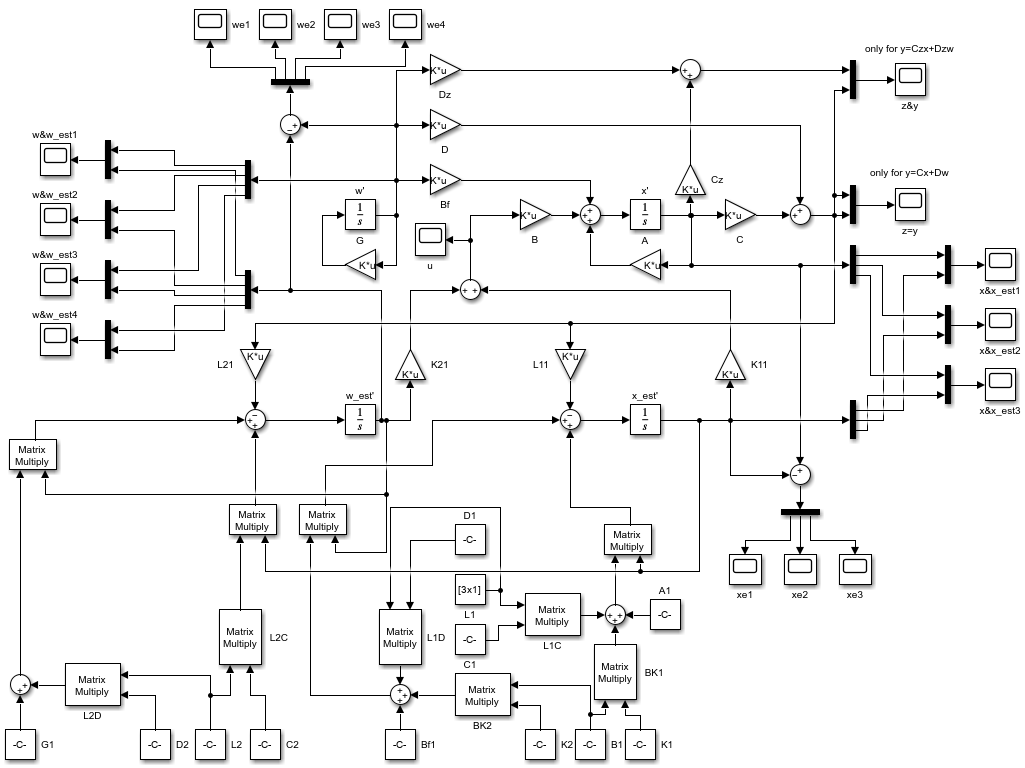
\includegraphics[scale=0.55]{3task_scheme.png}
        \captionsetup{skip=0pt}
        \caption{Схема моделирования системы для слежения и компенсации по выходу}
        \label{fig:3task_scheme}
    \end{figure}


    \subsection{Исследование системы перед синтезом регулятора}
    Матрицы $A,B$ такие же, как в первом задании. Имеем
    $$
    \sigma\left( A \right)=\left\{ -2,2\pm i \right\},\ A_{J_{re}}=\begin{bmatrix}
        -2     &0     &0\\
        0     &2     &1\\
        0    &-1     &2
        \end{bmatrix},\ B_{J_{re}}=\begin{bmatrix}
        0\\
         3\\
        -1
        \end{bmatrix};
    $$
    Система не полностью управляема,
    стабилизируема. Максимальная степень устойчивости $\alpha=2$.


    \subsection{Синтез компоненты обратной связи}
    Аналогично заданию 1 синтезируем $K_1$ при помощи матричного
    уравнения типа Риккати. Матрицы, участвующие в расчетах, не изменились.
    Тогда, получаем
    $$
    K_1=\begin{bmatrix}
    1.6000  &-11.2000    &1.6000
    \end{bmatrix},\
    \sigma\left( A+BK_1 \right)=\left\{ -2,-2.0000 \pm 4.1231i \right\};
    $$
    В первом задании уже выяснили, что регулятор синтезирован корректно.


    \subsection{Синтез матрицы коррекции наблюдателя}
    Матрицу наблюдателя $\mathcal{L}$ будем искать с помощью матричных неравенств
    $$
    Q\succ0,\ \mathcal{A}^TQ+Q\mathcal{A}+2\alpha Q+\mathcal{C}^TY^T+Y\mathcal{C}\prec 0,\ \mathcal{L}=Q^{-1}Y
    $$
    совместно с решением задачи минимизации управления. Зададим $\alpha=1$. Используя \texttt{cvx}, получаем
    $$
    \mathcal{L}=\begin{bmatrix}
        41.4979\\
   31.3700\\
  -30.9945\\
    0.2455\\
    1.4359\\
    1.1914\\
    0.6445
    \end{bmatrix}=\begin{bmatrix}
        L_1\\L_2
    \end{bmatrix}\Rightarrow L_1=\begin{bmatrix}
        41.4979\\
   31.3700\\
  -30.9945
    \end{bmatrix},\ L_2=\begin{bmatrix}
        0.2455\\
    1.4359\\
    1.1914\\
    0.6445
    \end{bmatrix};\ \mu=28.1390;
    $$
    Проверим собственные числа замкнутой системы $\mathcal{A}+\mathcal{L}\mathcal{C}$
    $$
    \sigma\left( \mathcal{A}+\mathcal{L}\mathcal{C} \right)=\left\{\begin{matrix}
        -1.4717\\
        -1.0103 \pm 3.3960i\\
        -1.0300 \pm 1.7041i\\
        -1.0850 \pm 0.3955i
    \end{matrix}\right\}
    $$
    Наблюдатель синтезирован корректно.


    \subsection{Синтез компоненты прямой связи следящего регулятора}
    Синтезируем $K_2$ для различных виртуальных выходов. Рассмотрим
    \begin{align*}
        &z_{1}=C_Zx+D_Zw\\
        &z_{2}=y=Cx+Dw
    \end{align*}
    Синтез возможен в том случае,
    если матрицы $A+BK_1$ и $\mathcal{A}+\mathcal{L}\mathcal{C}$ гурвицевы.
    В нашем случае условия выполнены -- мы проверяли собственные числа
    этих замкнутых систем ранее -- спектры матриц принадлежат левой комплексной полуплоскости.
    Процедура синтеза аналогична заданию 1. Получаем
    $$
    K_{2_{z1}}=\begin{bmatrix}
        -41.1631   &-9.8092   &27.7538  &-19.4769
    \end{bmatrix},
    $$
    $$
    K_{2_{z2}}=\begin{bmatrix}
        20.3076    &2.7419  &-14.2967    &8.5001
    \end{bmatrix};
    $$


    \subsection{Принцип внутренней модели}
    Если измеряемый выход $y$ равен регулируемому выходу $z$, и если
    регулятор обеспечивает устойчивость объекта в случае $w\equiv0$,
    то для решения задачи слежения и компенсации $\left( z\to0 \right)$
    необходимо, чтобы $$\sigma\left( \Gamma \right)\in\sigma\left( \bar{A} \right)$$
    Спектр матрицы $\Gamma$ мы уже находили
    $$
    \sigma\left( \Gamma \right)=\left\{ \pm i, \pm 3i \right\}
    $$
    Проверим спектры матриц $\bar{A}_{z_1}$ и $\bar{A}_{z_2}$. Матрицу $\bar{A}$
    выводили ранее (\ref{eq:barA}), когда представляли уравнения регулятора в форме
    В-С-В (\ref{eq:in_state_out}) с $y(t)$ как входом, $u(t)$ как выходом. Получаем
    $$
    \sigma\left( \bar{A}_{z_1} \right)=\left\{\begin{matrix}
        -1.9996\\
        -6.8702 \pm32.8647i\\
        0.0175 \pm 3.0096i\\
        -0.0085 \pm 0.9756i
    \end{matrix}\right\},\ \sigma\left( \bar{A}_{z_2} \right)=\left\{\begin{matrix}
        -1.9996\\
        -6.8613 \pm32.8152i\\
        \pm3.0000i\\
        \pm1.0000i
    \end{matrix}\right\};
    $$
    Для $z_1=C_Zx+D_Zw$ принцип внутренней модели не выполняется, для
    $z_2=Cx+Dw$ -- выполняется. Регулятор $K_{2_{z2}}$ умеет воспроизводить
    сигналы, за которыми надо проследить или которые нужно компенсировать.


    \subsection{Компьютерное моделирование}
    Выполним компьютерное моделирование для $K_{2_{z1}}$ и $K_{2_{z2}}$
    с нулевыми начальными условиями наблюдателя. Построим график
    формируемого регулятором управления $u(t)$, сравнительные графики
    $\begin{bmatrix}
        x(t)\\w(t)
    \end{bmatrix}$ и $\begin{bmatrix}
        \hat{x}(t)\\ \hat{w}(t)
    \end{bmatrix}$, график ошибки наблюдателя $e(t)=\begin{bmatrix}
        x(t)\\w(t)
    \end{bmatrix}-\begin{bmatrix}
        \hat{x}(t)\\ \hat{w}(t)
    \end{bmatrix}$ и сравнительные графики фактического и виртуального выходов $y(t)$ и $z(t)$
    ...


    \subsection{Вывод}
    ...


    \section{Общий вывод по работе}
    ...


    \section{Приложения}
    \subsection{Приложение 1}
    \begin{lstlisting}[label=task1, caption={Программа для задания 1}]
    % plant parameters
    A = [5 2 7;
         2 1 2;
        -2 -3 -4];
    B = [3; 1; -1];
    Bf = [-4 0 0 -1;
          0 0 0 0;
          4 0 0 0];

    G = [25 6 -20 11;
         14 3 -10 4;
         40 11 -31 17;
         6 4 -4 3];

    Cz = [-2 1 -1];
    D = 0;

    % G eigenvalues
    G_eig = eig(G)

    % A eigenvalues
    A_eig = eig(A)

    % Jordan matrix
    [Aj, J] = jordan(A);
    Pjre(:,1) = Aj(:,1);
    Pjre(:,2) = imag(Aj(:,2));
    Pjre(:,3) = real(Aj(:,3))
    Pjre_inv = Pjre^-1
    Aj_re = Pjre_inv * A * Pjre
    B_jre = Pjre_inv * B

    % solving Riccati
    Q = 0;
    v = 2;
    R = 1;
    a = 2;

    Aa = A + eye(3) * a;
    [Pk,K,e]=icare(Aa,sqrt(2)*B,Q,R);
    K1=-inv(R)*B'*Pk
    eK1=eig(A+B*K1)

    % K2 regulator synthesis
    cvx_begin sdp
    variable P(3,4)
    variable Y(1,4)
    P*G-A*P == B*Y+Bf;
    Cz*P + D == 0;
    cvx_end

    K2 = Y-K1*P
    \end{lstlisting}


    \subsection{Приложение 2}
    \begin{lstlisting}[label=task2, caption={Программа для задания 2}]
    % plant parameters
    A = [5 2 7;
         2 1 2;
        -2 -3 -4];
    B = [3; 1; -1];
    Bg = 0;

    G = [25 6 -20 11;
         14 3 -10 4;
         40 11 -31 17;
         6 4 -4 3];

    Cz = [-2 1 -1];
    Dz = [-20 -6 16 -9];

    % solving Riccati
    Q = 0;
    v = 2;
    R = 1;
    a = 2;

    Aa = A + eye(3) * a;
    [Pk,K,e]=icare(Aa,sqrt(2)*B,Q,R);
    K1=-inv(R)*B'*Pk
    eK1=eig(A+B*K1)

    % K2 regulator synthesis
    cvx_begin sdp
    variable P(3,4)
    variable Y(1,4)
    P*G-A*P == B*Y+Bg;
    Cz*P + Dz == 0;
    cvx_end

    K2 = Y-K1*P
    \end{lstlisting}


    \subsection{Приложение 3}
    \begin{lstlisting}[label=task3, caption={Программа для задания 3}]
    % plant parameters
    A = [5 2 7;
         2 1 2;
        -2 -3 -4];
    B = [3; 1; -1];
    Bf = [-4 0 0 -1;
          0 0 0 0;
          4 0 0 0];

    G = [25 6 -20 11;
         14 3 -10 4;
         40 11 -31 17;
         6 4 -4 3];

    Cz = [-2 1 -1];
    Dz = [-20 -6 16 -9];

    C = [2 0 3];
    D = [8 2 -6 4];

    % matrices
    bigC = [C D];
    bigA = [A Bf;
            zeros(4,3) G];

    % eig bigA
    eig_bigA = eig(bigA)

    % re jordan
    [P, J] = jordan(bigA);
    P_re(:,1) = P(:,1);
    P_re(:,2) = imag(P(:,2));
    P_re(:,3) = real(P(:,3));
    P_re(:,4) = imag(P(:,4));
    P_re(:,5) = real(P(:,5));
    P_re(:,6) = imag(P(:,6));
    P_re(:,7) = real(P(:,7))
    Pre_inv = P_re^-1
    bigA_J_re = Pre_inv * bigA * P_re
    C_J_re = bigC * P_re

    % solving Riccati
    Q = 0;
    v = 2;
    R = 1;
    a = 2;

    Aa = A + eye(3) * a;
    [Pk,K,e]=icare(Aa,sqrt(2)*B,Q,R);
    K1=-inv(R)*B'*Pk
    eK1=eig(A+B*K1)

    % find L: solving LMI with control constraint
    al = 1;
    xw0=[0;0;0;1;1;1;1];
    xw0_est=[0;0;0;0;0;0;0];
    xwe0=xw0-xw0_est;

    cvx_begin sdp
    variable Q(7,7)
    variable Y(7,1)
    variable mumu
    minimize mumu
    Q>0.0001*eye(7);
    bigA'*Q + Q*bigA+ 2*al*Q + bigC'*Y' + Y*bigC <= 0;
    [Q xwe0;
     xwe0' 1]>0;
    [Q Y;
     Y' mumu]>0;
    cvx_end
    mu = sqrt(mumu)
    bigL=inv(Q)*Y
    e_bigL=eig(bigA+bigL*bigC)

    % K2_CD regulator synthesis
    cvx_begin sdp
    variable P1(3,4)
    variable Y1(1,4)
    P1*G-A*P1 == B*Y1+Bf;
    C*P1 + D == 0;
    cvx_end

    K2_CD = Y1-K1*P1

    % K2_CzDz regulator synthesis
    cvx_begin sdp
    variable P2(3,4)
    variable Y2(1,4)
    P2*G-A*P2 == B*Y2+Bf;
    Cz*P2 + Dz == 0;
    cvx_end

    K2_CzDz = Y2-K1*P2

    L1 = [bigL(1); bigL(2); bigL(3)]
    L2 = [bigL(4); bigL(5); bigL(6); bigL(7)]

    % the principle of the internal model
    eig_G = eig(G)
    bar_A_CD = [A+B*K1+L1*C B*K2_CD+Bf+L1*D;
                L2*C G+L2*D]
    bar_A_CzDz = [A+B*K1+L1*C B*K2_CzDz+Bf+L1*D;
                  L2*C G+L2*D]
    eig_bar_A_CD = eig(bar_A_CD)
    eig_bar_A_CzDz = eig(bar_A_CzDz)
    \end{lstlisting}
\end{document}